
%%%%%%%%%%%%%%%%%%%%%%% file typeinst.tex %%%%%%%%%%%%%%%%%%%%%%%%%
%
% This is the LaTeX source for the TDPTemplate using
% the LaTeX document class 'llncs.cls' Springer LNAI format
% used in the RoboCup Symposium submissions.
% http://www.springer.com/computer/lncs?SGWID=0-164-6-793341-0
%
% It may be used as a template for your own TDP - copy it
% to a new file with a new name and use it as the basis
% for your Team Description Paper
%
% NB: the document class 'llncs' has its own and detailed documentation, see
% ftp://ftp.springer.de/data/pubftp/pub/tex/latex/llncs/latex2e/llncsdoc.pdf
%
%%%%%%%%%%%%%%%%%%%%%%%%%%%%%%%%%%%%%%%%%%%%%%%%%%%%%%%%%%%%%%%%%%%

\documentclass[runningheads,a4paper]{llncs}
\usepackage{amssymb}
\setcounter{tocdepth}{3}
\usepackage{graphicx}
\usepackage{amssymb}
\usepackage[utf8]{inputenc}
\usepackage{url}
\usepackage{float}
\usepackage{amsmath}
\usepackage{graphicx}
\usepackage{wrapfig}
\usepackage{tabto}
\usepackage{lipsum}
\usepackage[table,xcdraw]{xcolor}

\begin{document}

\title{Walking Machine @Home \newline \: 2017 Team Description Paper}

\author{Jeffrey Cousineau et al.}
\institute{École de Technologie Supérieure \\ 1100 rue Notre-Dame Ouest, Montreal, QC, Canada H3C 1K3 \\
\texttt{http://walkingmachine.ca,} \texttt{walking@ens.etsmtl.ca,} \texttt{https://github.com/WalkingMachine}}
\maketitle


%%%%%%%%%%%%%%%%%%%%%%%%%%%%%%%%%%%%%%%%%%%%%%%%%%%%%%%%%%%%%%%%%%%%%%%%%%%%%%%%%%%%

\begin{abstract}

This paper gives details about the RoboCup@Home league team Walking Machine, from ETS University in Montreal, Canada for the next competition in Nagoya, Japan, in July 2017. The robot from Walking Machine, named SARA for "Système d’Assistance Robotique Autonome" (in English, Automated Robotic Assistance System), is a robot entirely built by the scientific club from ETS, mainly composed of undergraduates students. The robot is used for social interaction with humans, navigation and object manipulation. This document shows the electrical, mechanical and software properties and functionalities of SARA. It specifically emphasises on human following, object and people recognition as well as navigation, manipulation and human-robot interaction.

\end{abstract}

%%%%%%%%%%%%%%%%%%%%%%%%%%%%%%%%%%%%%%%%%%%%%%%%%%%%%%%%%%%%%%%%%%%%%%%%%%%%%%%%%%%%

\section{Introduction}
\tab Walking Machine’s team is a young team from Montreal, Quebec, in Canada, composed of engineering student in the field of mechanical, electrical and software engineering. We have been working on our robot for the last year in prevision of the Robocup at Home competition. As this is our second participation, we learned a lot on our first attempt last year and have made various modifications to get better results. In the past, the team went in many competitions like the Eurobot, but made the leap for the RoboCup@Home competition to get a bigger challenge. \\

SARA, our creation, was designed for polyvalent human-robot interaction as well as efficient navigation and object manipulation. Our robot is mounted on four mecanum wheels powered by Roboteq drives, has one arm mimicking a normal human arm, and sensors for communication and navigation. Our team has developed knowledge in object and people detection/recognition, as well as navigation using a laser scanner, odometry on the wheels and a Asus Xtion camera. All of these parts are interfaced through ROS (Robot Operating System). \\

\section{Electrical and mechanical design of SARA}
\subsection{Electrical}
\tab The electrical design was mostly done using pre-built electrical assets. For example, we use Roboteq drives to power Maxon motors. The robot can run at more than 1 m/s in automatic navigation mode. The feedback of the motor speed is done with precise optical encoders and the drive control the motor speed with a PID algorithm. \\

SARA uses lithium-ion power cells with built-in voltage balancing. Each cell has a nominal voltage of 4.2 volts and, once linked together, offers a supply of 25.2 volts to the robot systems. This year, we conceived a new battery which is smaller than last year but gives us the possibility to be swap, so we get two times the capacity. The health of the battery system is monitored with a custom BMS (Battery Monitoring System) developed by our team. An emergency stop is linked directly to the battery to cut any power if something should go bad. Moreover, a motion stop is being developed to stop the robot during any dangerous action. A custom power distribution board was made by our team to provide enough power to the lidar, the gripper, the arm and the various embedded computer. \\
\begin{figure}
  \centering
  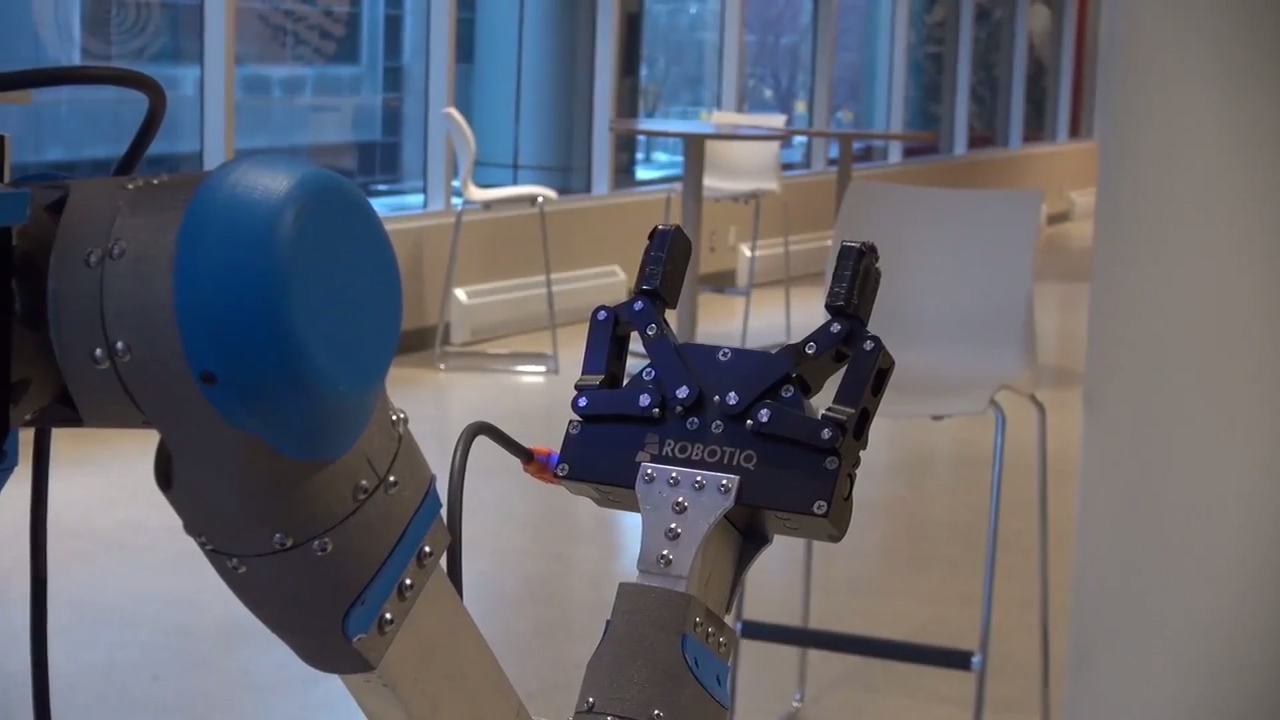
\includegraphics[width=150pt]{images/robotiq.png}
  \caption{Robotiq gripper}
\end{figure}\\
The robot uses sensors like a laser sensor for 2D mapping and leg tracking as well as Xtion camera for body tracking. The camera also provides depth perception to recognize objects and faces. We are also currently implementing the kinect 2 for future uses. The face of the robot was developed by the team and use Neopixel RGB LEDs to provide a range of possible emotions and is also linked to voice, so the LEDs will modulate the opening of the mouth according to the voice of SARA when she's talking. 

\subsection{Mechanical}
\tab The general design of the robot is made of a ground base, a trunk, a robotic arm and the head which include a motion sensor, a microphone and a DEL face matrix. The basic frame is assembled with aluminum sheet metal. The shells are made from prototyping plastics, and also with acrylic sheets. We made a significant weight loss this year since we change the main desktop pc for a laptop and the battery reduction also take away some of this weight.  \\

One of the principal interests of the robot is its omni-directional wheels. The 45 angle of each roller on the wheel allows frontal displacements as well as lateral movements. The only thing we control are the angular speed and the rotational direction of all the DC motors connected to each wheel. \\

Our main base has been rethink and redesign to be smaller. This decision lead to a better navigation because we experienced some difficulties to go through door with our old base due to his dimensions being too large. We took advantage of this redesign to build a frame that with easy changing compartments for the electric system and the computer. \\

An innovation is also made on this robot with the titanium printed arm. Considering the high power of the arm actuators, a decision has been taken to use a high performance factor metal to lift the biggest load as possible without any break. Moreover, this metal should be printed to make the fabrication easier. This arm was entirely designed with finite elements method to optimize the resistance and ensure required stiffness, as it is possible to see in figure 2. \\

This specific arm has currently five DOF (Degrees Of Freedom) but will soon have 7 with the add of two other links. This will give us more liberty and help us get to harder to reach objects. The motors used are the same as the JACO arm model from Kinova and use harmonic drive, which give us an extreme precision. The arm, once fixed to SARA’s frame, can lift up to 2kgs at full extension. Each motor is linked in series and receives its power from the one before. The arm is controlled by a JACO arm base, which distributes commands to the motors to move them. \\

\section{Environment perception}
\subsection{Navigation}
\tab Most of the software development is toward the movements of the robot in its environment. For this, SARA can build a 2D map using a laser scanner. Using the simultaneous localization and mapping (SLAM) method she can build a 2D map while exploring it and simultaneously know where she is in using the odometry on her wheels, the inertial measurement unit (IMU) was also implement this year for a better localization. We also implemented, base on the robot\_pose\_efk ROS package \cite{poseefk}, a kalman filter to get a better pose estimation of our robot. \\
\begin{figure}
  \centering
  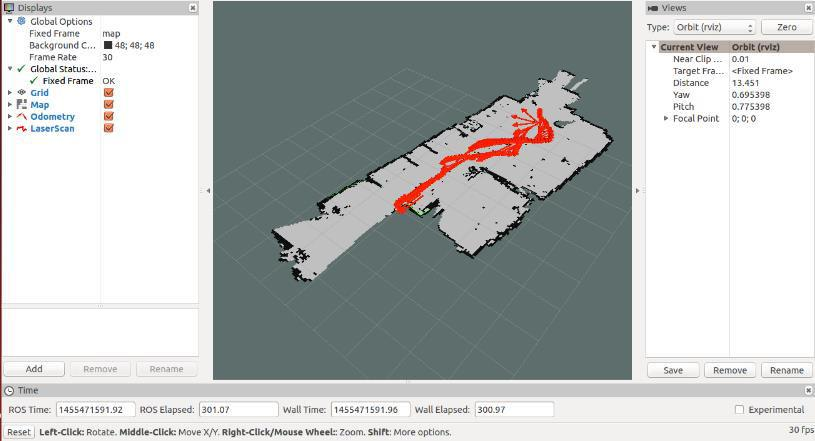
\includegraphics[width=150pt]{images/map.jpg}
  \caption{Mapping}
\end{figure}\\
Using the sensor, the robot builds a 2D map, which can be saved and then sent to the part of the software responsible of moving the base of the robot. The 2D map updates itself often to be able to react to fast-changing environment, such as an object thrown in front of the robot.



\subsection{People and objects perception}
\tab An RGB/IR Asus Xtion camera is used in parallel with the Hokuyo to build a 3D map of the environment, but at this point we integrated only the 2D mapping and are using the Xtion camera for object and people recognition. Knowing the distances from the base of the robot to the camera, it is possible to use body tracking, which means the robot detects a human body and can analyze it to know where its head, shoulders, hands, legs and feet are. The robot will be able to interpret specific movements using this. \\

Face recognition is done through the Xtion. It is possible to add new people via specific services of the software. The face recognition differentiate people through banks of images of the faces and depths of the multiple points. Using statistical analysis, it goes through the bank of images when somebody is presented to the robot and assigns the most reliable face if a match is
possible, else the new person is unknown. \\

For objects recognition, we decided to use object recognition kitchen combine (ORK) to the Kinect V2, which give us a good quality pointcloud. As undergraduates students, we tough that using ORK would be a good alternative as we don't have the required experience to developed our own object recognition algorithm. This package gives us very powerful tools to detect 3D objects in an environment. \\

\begin{figure}
  \centering
  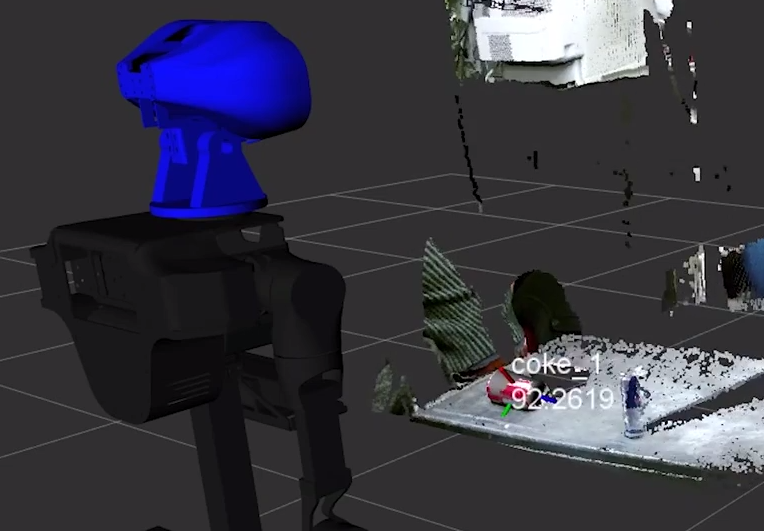
\includegraphics[width=150pt]{images/objectreco.png}
  \caption{Object recognition}
\end{figure}

\newpage
\section{Decision making}
\tab Our high level decision making is made by a hierarchical finite state machine (HFSM). At the highest level, the HFSM wait for an order. Once an order is received, it switches to the corresponding state. It then enters a lower FSM that describe in details all the steps to execute the task. 

\subsection{Navigation}
\tab Autonomous navigation uses the Navigation package from ROS. This package is composed of many algorithms that allow a robot to localize itself in a map, plan a trajectory to reach a given target position and compute velocity command. A planar laser scanner and velocity readings are used to build the map. A particle filter tracks the position of the robot as it moves. Velocity commands are computed by the main algorithm and are then sent to the wheels. 

\subsection{Object manipulation}
\tab First of all, a model of the manipulator was created by using the Denavit-Hartenberg \cite{kinematic} parameters. These parameters allow to compute the transform matrix between different reference frames. Using sensor stream from the stereoscopic camera, the robot is able to locate objects and register their position in its coordinate frame. The object pose becomes the manipulator's end effector's target pose. Inverse kinematics is computed using the Cyclic Coordinate Descent (CCD) method \cite{coordinate}. Starting at the most distal joint and for each joint, this iterative method computes the movement required to minimize the alignment error between the joint pose to effector pose vector and the joint pose to target pose vector. Joint position adjustments are made until the end effector is within tolerance or the maximum number of iterations is reached. Considering only one joint at time reduces the complexity of the problem while making the algorithm robust against singularities \cite{springer}. 
\begin{wrapfigure}{R}{0.3\textwidth}
\centering
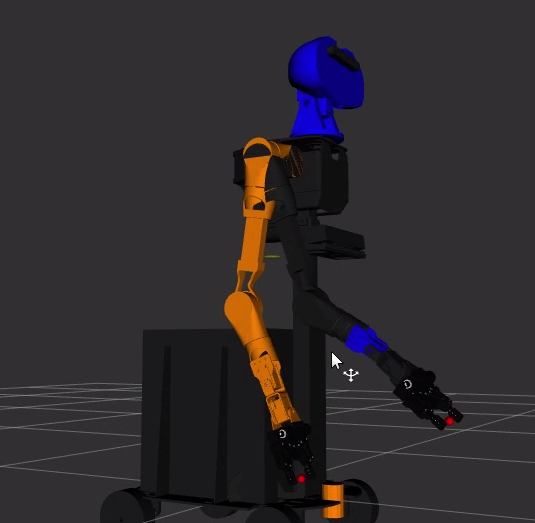
\includegraphics[width=0.25\textwidth]{images/arm_sim.png}
\caption{Arm simulation}
\end{wrapfigure}

\newpage
\subsection{Human-robot interaction}
\tab SARA has voice recognition package which branches directly in the decision making part. She has multiple pre-made voice command that she can understand and each of this command will need to be enabled beforehand by saying her name. Each time SARA hears her name, she will switch in command waiting mode. If the said command is available in her vocal commands tree, she will demand confirmation of it and then proceed on. At any time during an action, she can give details on what she is doing and can be stopped by the safe word STOP. This command overrides every other and acts as a software stop. She uses a speech synthesis package that we embedded in ROS known as SVOX pico2wave \cite{svox}, to express herself according to her state.\\

Giving that our robot need to achieved a higher level of autonomy, we had to integrate some language syntactic analysis, which we call semantic analysing. Since we can't have only pre-made voice command, we decided to use LU4R \cite{lu4r} made by University of Rome. This give us the possibility to extract main topics in a sentence and then, our robot can act according to these topics. For this to work, we also have to give as parameter a description of our semantic map. This means, using KnowRob, we analyse the whole map and extract the localisation of every object in a specific room. Furthermore, we use this information to have a better understanding of our environment, which is complementary to the LU4R sentence analysis.


\section{Conclusions and future work}
\tab As you can see, since last year, we made several progress, starting with the improvement of our object detection module. Also, the implementation of a semantic representation of the environment is a big step for us since it helps our robot to have a better understanding of his surrounding. Finally, the various mechanicals modifications will help for a better navigation and a better management of our robot. So SARA is now a complete autonomous system able of interaction with the human as well as navigation in her environment. Using his multiple sensors, like laser sensor, depth camera, IMU and odometry our robot can analyze his environment, recognize people and objects and navigate through obstacles. It can then interact with objects and people using his voice recognition and voice synthesis abilities to keep track of his state. All of the requirements for the Robocup@home are met by SARA and it's a fast-evolving robot considering the team is really young and composed of undergraduates in various engineering programs. As future works, we will add a second arm to give us the possibility for two-hands manipulation. Also, we'll add vertical translation to our body to give our robot a larger range for objects manipulation.

\section*{Robot SARA Hardware Description}
% TODO Change picture and description
Specifications for robot SARA are as follows:

\begin{table}

\label{my-label}

\begin{tabular}{l|p{90mm}}
\hline
\rowcolor[HTML]{FFFFFF} 
\multicolumn{2}{c}{\cellcolor[HTML]{FFFFFF}\textbf{SARA}}                                                      \\ \hline
\rowcolor[HTML]{EAEFF6} 
\textbf{Base}               & Custom base with fully holonomic platform                                        \\
\rowcolor[HTML]{FFFFFF} 
\textbf{Right arm}          & 7 DoF custom arm made of Kinova motors                                           \\
\rowcolor[HTML]{EAEFF6} 
\textbf{Neck}               & Tilt and pan unit using two Dynamixel MX-64R servo actuator                      \\
\rowcolor[HTML]{FFFFFF} 
\textbf{Head}               & Custom head made of RGB neopixels leds and Asus Xtion Pro                        \\
\rowcolor[HTML]{EAEFF6} 
\textbf{Gripper}            & Robotiq 2 fingers 140mm                                                           \\
\rowcolor[HTML]{FFFFFF}
\textbf{Dimensions}         & \begin{tabular}[c]{@{}l@{}}Base : 0,61m. X 0,77m.\\ Height : 1,68m.\end{tabular} \\
\rowcolor[HTML]{EAEFF6} 
\textbf{Weight}             & $\sim$60kg                                                                      \\
\rowcolor[HTML]{FFFFFF} 
\textbf{Additional sensors} & Hokuyo UTM-30LX on base                                                          \\
\rowcolor[HTML]{EAEFF6} 
\textbf{Microphone}         & Rode microphone											                         \\
\rowcolor[HTML]{FFFFFF} 
\textbf{Batteries}          & 2x 20V Dewalt drill battery 5aH                                                 \\
\rowcolor[HTML]{EAEFF6} 
\textbf{Computer}           & 1x Lenovo p50 with 32GB RAM and nVidia Quadro M2000 4GB, 1x Raspberry Pi 3       \\ \hline
\end{tabular}
\caption{Robot's hardware description}
\end{table}
\begin{wrapfigure}[10]{r}{0.25\textwidth}
	\centering
	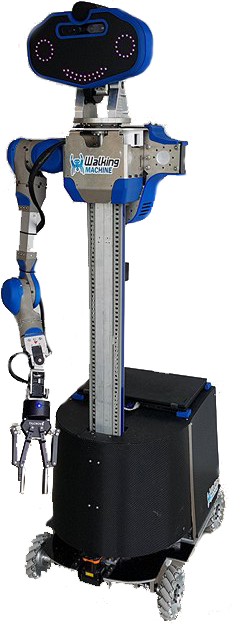
\includegraphics[width=0.30\textwidth]{images/sara_2.png}
	\caption{Robot SARA}
\end{wrapfigure}
\section*{Robot's Software Description}

For our robot we are using the following software:

\begin{itemize}
	\item Platform: Robotic Operating System (ROS) Kinetic on Ubuntu 16.04
	\item Navigation, localization and mapping: \href{http://wiki.ros.org/gmapping}{Gmapping}, \href{http://wiki.ros.org/amcl}{AMCL}, \href{http://wiki.ros.org/pointcloud_to_laserscan}{pointcloud\_to\_laserscan}
	\item Face recognition: \href{http://wiki.ros.org/people}{People}
	\item Speech recognition: \href{https://github.com/WalkingMachine/lab_ros_speech_to_text}{Google Speech API}
	\item Speech comprehension: \href{http://sag.art.uniroma2.it/lu4r.html}{LU4R}, \href{https://github.com/WalkingMachine/lu4r_ros}{lu4r\_ros}
	\item Speech generation: \href{https://doc.ubuntu-fr.org/svoxpico}{Svoxpico}
	\item Object recognition: \href{https://github.com/WalkingMachine/wm_darknet}{Darknet with YOLO v2 }
	\item Arm control: \href{http://wiki.ros.org/moveit}{MoveIt} and \href{https://github.com/Kinovarobotics/kinova-ros}{Kinova API}
	\item Task executor: \href{http://wiki.ros.org/flexbe}{Flexbe} 
	\item World reprensentation: \href{http://github.com/walkingmachine/wonderland}{Wonderland}
\end{itemize}
	

\section*{Team members}
Jeffrey Cousineau, Maxime St-Pierre, Jonathan Fortin, Thierry Pouplier, Alexandre Doyle, Jimmy Poirier, Cassandra Lépine, Philippe La Madelaine, Samuel Otis, Redouane Laref, Louis-Charle Labarre, Francis Grégoire, Simon Landry, Aloïs Goudard-Bellissens, Lucas Maurice, Léonore Jean-François, Nicolas Nadeau, Daniel Sami, Alexandre Salconi-Denis, Quentin Bourret, Laureline Estivalet, Julien Côté 

\nocite{*}
\bibliographystyle{plain}
\bibliography{references}


\end{document} 
